\documentclass{beamer}
\mode<presentation>
\usetheme{CambridgeUS}
\usepackage[russian]{babel}
\usepackage[utf8]{inputenc}
\usepackage[T2A]{fontenc}
\usepackage{sansmathaccent}

\usepackage{verbatim}
\usepackage{alltt}
\usepackage{minted}

\pdfmapfile{+sansmathaccent.map}
\title[Деревья]{Деревья: бинарные, декартовы, сбалансированные}
\author{Наумов Д.А., доц. каф. КТ}
\date[12.04.2021] {Алгоритмы и структуры данных, 2021}

\begin{document}

%ТИТУЛЬНЫЙ СЛАЙД
\begin{frame}
  \titlepage
\end{frame}
  
%СОДЕРЖАНИЕ ЛЕКЦИИ
\begin{frame}
  \frametitle{Содержание лекции}
  \tableofcontents  
\end{frame}

\section{Абстракция \textit{отображение}}
  
\begin{frame}[t]
	\begin{block}{Отображение}
		 абстракция, устанавливающая направленное соответствие между двумя множествами (множеством ключей и множеством данных) и реализующая над ними определённые операции. 
	\end{block}	
	\begin{figure}[h]
		\centering
		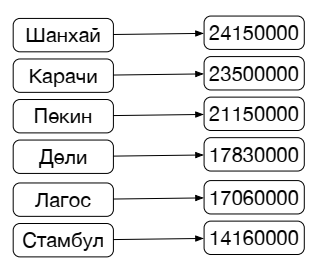
\includegraphics[scale=0.5]{images/lec07-pic01.png}
		\caption{Пример отображения: каждому городу соответствует численность его населения}
	\end{figure}
\end{frame}	

\begin{frame}[t]	
	Абстракция \textit{отображение} есть аналог дискретной функции:
	\begin{block}{Функция}
		 есть отображение множества D на множество E. 
	\end{block}
	\begin{figure}[h]
		\centering
		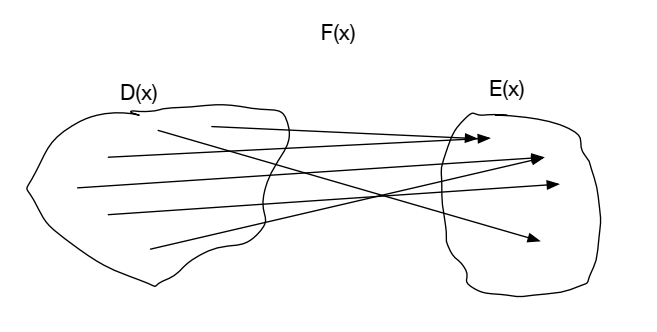
\includegraphics[scale=0.5]{images/lec07-pic02.png}
		\caption{Отображение множества D на множество E}
	\end{figure}
\end{frame}
 
\begin{frame}[fragile, t]	
	Наша цель -- реализовать некий \textit{словарь}, в котором мы можем добавлять, искать и удалять \textit{словарные статьи}.

	~
	
	C++, наряду с другими современными языками, предоставляет возможность использовать отображения как обобщение понятия массив с помощью синтаксиса индексации:
	\begin{minted}{c}
map m<string,int>;
m["Шанхай"] = 24150000;
m["Карачи"] = 23500000;
m["Пекин"] = 21150000;
m["Дели"] = 17830000;
...
int BeijingPopulation = m["Пекин"];
...
for (auto x: m) {
  printf("Population of %s is %d\n", x.first, x.second);
}	
	\end{minted}
\end{frame} 

\begin{frame}[t]{Интерфейс абстракции \textit{отображение}}
	Интерфейс абстракции отображение есть частный случай абстракции хранилища CRUD (create, read, update, delete):
	\begin{itemize}
		\item insert(key, value) -- добавить элемент с ключом key и значением value.
		\item Item find(key) -- найти элемент с ключом key и вернуть его.
		\item erase(key) -- удалить элемент с ключом key.
		\item walk -- получить все ключи (или все пары ключ/значение) в каком-либо порядке.
	\end{itemize}		
	В дальнейшем под термином ключ мы понимаем пару \textit{ключ+значение}, в которой определена операция сравнения по ключу.

	~
	Абстракцию \textit{множество} можно рассматривать как частный случай абстракции отображение.
	\begin{itemize}
		\item множество ключей с прикрепленными данными;
		\item отображение набора ключей на логические переменные.
	\end{itemize}
\end{frame}

\section{Бинарные деревья поиска}
  
\begin{frame}[t]
	\begin{block}{Бинарным деревом поиска (Binary SearchTree, BST)}
		 называется бинарное дерево, в котором все узлы, находящиеся справа от родителя, имеют значения, не меньшие значения в родительском узле, а слева — не большие этого значения. 
	\end{block}	
	\textbf{Задача}. 
	\begin{itemize}
		\item На вход подаётся последовательность чисел. 
		\item Выходом должно быть двоичное дерево поиска.
	\end{itemize}	
	\begin{figure}[h]
		\centering
		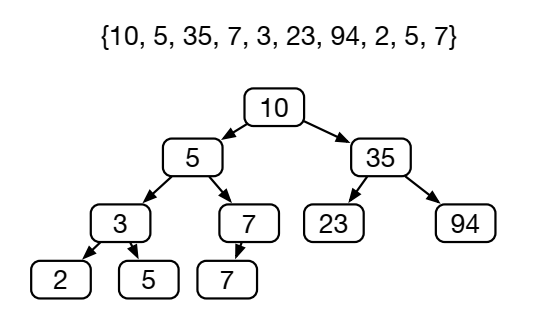
\includegraphics[scale=0.5]{images/lec07-pic03.png}
		\caption{Пример BST}
	\end{figure}
\end{frame}	

\begin{frame}{Алгоритм поиска элемента в BST, содержащего ключ X}
	\begin{enumerate}
		\item Делаем текущий узел корневым.
		\item Переходим в текущий узел C.
		\item Если X = C:Key, то алгоритм завершён.
		\item Если X > C:Key и C имеет потомка справа, то делаем текущим узлом потомка справа. Переходим к п. 2.
		\item Если X < C:Key и C имеет потомка слева, то делаем текущим узлом потомка слева. Переходим к п. 2.
		\item Ключ не найден. Конец алгоритма.	
	\end{enumerate}
	Алгоритм прост и эффективен, и его сложность определяется только наибольшей высотой дер
\end{frame}	

\begin{frame}{Алгоритм \textit{наивного} построения BST}
	\begin{enumerate}
		\item Делаем текущий узел корневым.
		\item Переходим в текущий узел C.
		\item Если X = C:Key, то алгоритм завершён, вставка невозможна.
		\item Если X > C:Key и C имеет потомка справа, то делаем текущим узлом потомка справа. Переходим к п. 2.
		\item Если X > C:Key и C потомка справа не имеет, то создаём правого потомка с ключом X и завершаем алгоритм.
		\item Если X < C:Key и C имеет потомка слева, то делаем текущим узлом потомка слева. Переходим к п. 2.
		\item Если X < C:Key и C потомка слева не имеет, то создаём левого потомка с ключом X и завершаем алгоритм.
	\end{enumerate}	
\end{frame}	

\begin{frame}{Алгоритм \textit{наивного} построения BST}
	\begin{itemize}
		\item первый поступивший элемент последовательности формирует корневой узел дерева -- и каждый последующий элемент занимает соответствующее место после неудачного поиска (если поиск удачен, то дерево уже содержит ключ). 
		\item Неудачный поиск всегда заканчивается на каком-то узле, у которого в нужном направлении нет потомка.
	\end{itemize}
	\begin{figure}[h]
		\centering
		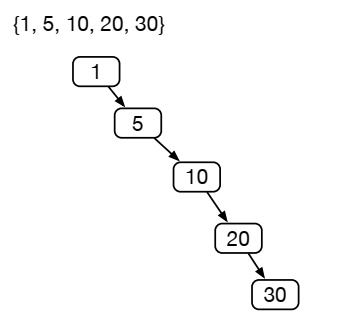
\includegraphics[scale=0.4]{images/lec07-pic04.png}
		\caption{Пример вырожденного BST}
	\end{figure}
\end{frame}	

\begin{frame}
	\begin{block}{Случайное бинарное дерево T размера n}
		 дерево, получающееся из пустого бинарного дерева поиска после добавления в него n узлов с различными ключами в случайном порядке, при условии, что все n! возможных последовательностей добавления равновероятны. 
	\end{block}	

	~	
	
	Средняя глубина случайного бинарного дерева: $d(N)=2 ln(N)$.

	~
	
	Cредние времена выполнения операций вставки, удаления и поиска в случайном бинарном дереве есть $\Theta(log_2(N))$.
\end{frame}

\begin{frame}[fragile]{Поиск минимального/максимального ключа}
	Так как все потомки слева от узла имеют значения ключей, меньшие значения ключа самого узла, то наименьший элемент всегда находится в самом низу левого поддерева. 

	~	
	
	Аналогично, наибольший элемент всегда находится в самом низу правого поддерева.
	
	\begin{minted}{c}
tree * minNode(tree *t) {
	if (t == nullptr) return nullptr;
	while (t->left != nullptr) {
		t = t->left;
	}
	return t;
}
	\end{minted}
	Методы поиска и вставки, описанные ранее, достаточно просты.
\end{frame}

\begin{frame}[fragile]{Удаление узла}
	Процедура удаления -- сложнее, требуется рассмотреть три случая:
	\begin{enumerate}
		\item У удаляемого узла нет потомков -- достаточно удалить этот узел у родителя.
		\item Имеется один потомок -- переставляем узел у родителя на потомка.
		\item Имеется два потомка -- находим самый левый лист в правом поддереве и им замещаем удаляемый.
	\end{enumerate}
\end{frame}

\begin{frame}[fragile]
	\textbf{Первый случай}. Удаление терминального узла 6.
	\begin{figure}[h]
		\centering
		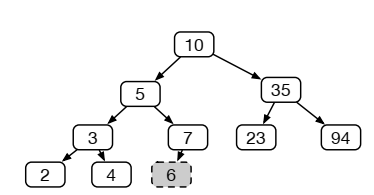
\includegraphics[scale=0.5]{images/lec07-pic05.png}
		\caption{До удаление}
	\end{figure}
	\begin{figure}[h]
		\centering
		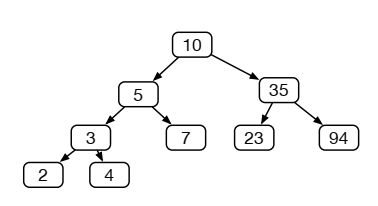
\includegraphics[scale=0.5]{images/lec07-pic06.png}
		\caption{После удаления}
	\end{figure}	
\end{frame}

\begin{frame}[fragile]
	\textbf{Второй случай}. Удаление узла 7, имеющего одного потомка.
	\begin{figure}[h]
		\centering
		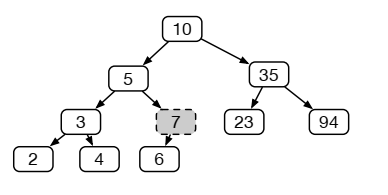
\includegraphics[scale=0.5]{images/lec07-pic07.png}
		\caption{До удаление}
	\end{figure}
	\begin{figure}[h]
		\centering
		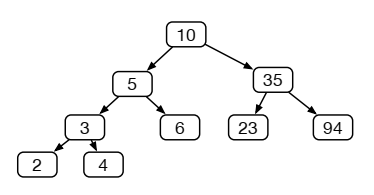
\includegraphics[scale=0.5]{images/lec07-pic08.png}
		\caption{После удаления. Единственный потомок занял место удаляемого узла}
	\end{figure}	
\end{frame}

\begin{frame}[fragile]
	\textbf{Третий случай}. Удаление узла 10, имеющего двух потомков.
	\begin{figure}[h]
		\centering
		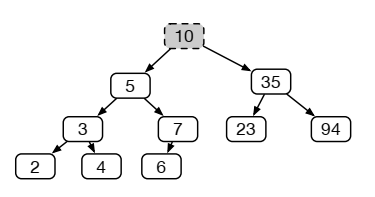
\includegraphics[scale=0.5]{images/lec07-pic09.png}
		\caption{До удаление}
	\end{figure}
	\begin{figure}[h]
		\centering
		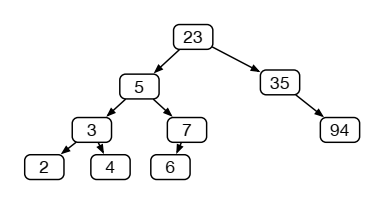
\includegraphics[scale=0.5]{images/lec07-pic10.png}
		\caption{После удаления. Самый левый потомок занял место удаляемого}
	\end{figure}	
\end{frame}

\begin{frame}[fragile]
	\begin{figure}[h]
		\centering
		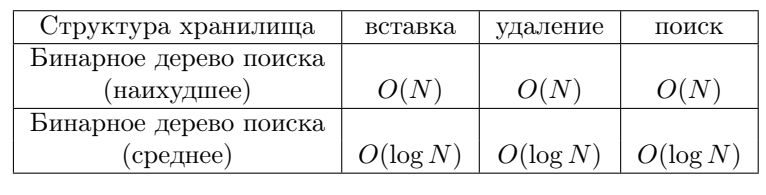
\includegraphics[scale=0.5]{images/lec07-pic11.png}
		\caption{Сложность операций для бинарного дерева поиска}
	\end{figure}
	
	\begin{itemize}
		\item Сложность всех алгоритмов в бинарных деревьях поиска определяется средневзвешенной глубиной. 
		\item Операции вставки/удаления могут привести к дисбалансу и ухудшению средних показателей. 
		\item Для борьбы с дисбалансом применяют \textit{рандомизацию} и \textit{балансировку}.
	\end{itemize}
\end{frame}

\begin{frame}[fragile]
	\begin{itemize}
		\item Cоздание BST из упорядоченной последовательности чревато крайне несбалансированным деревом. Возникает 		\item Вопрос: а что будет, если вставлять новые элементы не в терминальные узлы дерева, а заменять ими корень?
		\item Последствия таковы: если вставляемый элемент больше корня, то старый корень сделаем левым поддеревом, а его правое поддерево -- нашим правым поддеревом. 
		\item Аналогично рассуждаем для случая, когда вставляемый элемент меньше корня. К сожалению, и в том, и в другом случае может нарушиться упорядоченность. 
	\end{itemize}
\end{frame}

\begin{frame}[fragile]
	Чтобы нарушений не происходило, требуется сохранять инвариант упорядоченности. Для этого введём понятие \textbf{поворота}, не изменяющего упорядоченные свойства дерева, но меняющего его структуру, то есть высоту поддеревьев.
	\begin{itemize}
		\item H есть сокращение от слова Head, 
		\item L -- от Left 
		\item R -- от Right.
	\end{itemize}
	\begin{figure}[h]
		\centering
		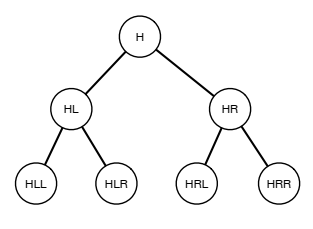
\includegraphics[scale=0.75]{images/lec07-pic12.png}
	\end{figure}
\end{frame}

\begin{frame}[fragile]
	После поворота направо дерево будет выглядеть так:
	\begin{figure}[h]
		\centering
		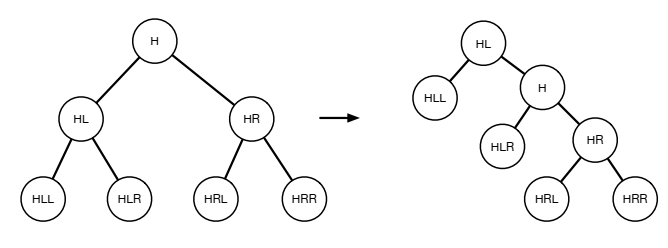
\includegraphics[scale=0.4]{images/lec07-pic13.png}
		\caption{BST: дерево после правого поворота}
	\end{figure}
	\begin{minted}{c}
void rotateRight(node* &head) {
	node *temp = head->left;
	head->left = temp->right;
	temp->right = head;
	head = temp;
}
	\end{minted}
\end{frame}

\begin{frame}[fragile]
	После поворота налево дерево будет выглядеть так:
	\begin{figure}[h]
		\centering
		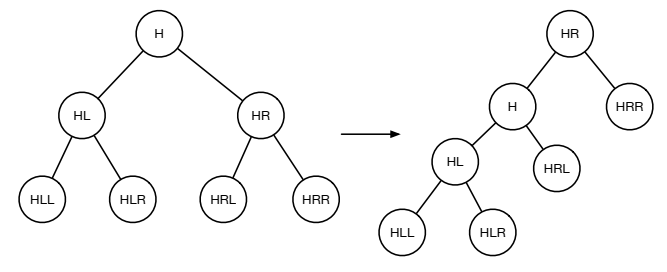
\includegraphics[scale=0.4]{images/lec07-pic14.png}
		\caption{BST: дерево после левого поворота}
	\end{figure}
	\begin{minted}{c}
void rotateLeft(node* &head) {
	node *temp = head->right;
	head->right = temp->left;
	temp->left = head;
	head = temp;
}
	\end{minted}
\end{frame}

\begin{frame}[fragile]
	Функция вставки нового узла в корень дерева:
	\begin{minted}{c}
void insert(node* &head, item x) {
	if (head == nullptr) {
		head = new node(x);
		return;
	}
	if (x.key < head->item->key) {
		insert(head->left, x);
		rotateRight(head);
	} else {
		insert(head->right, x);
		rotateLeft(head);
	}
}	
	\end{minted}
\end{frame}

\begin{frame}[fragile]{Рандомизированное дерево}
	\begin{itemize}
		\item Мы знаем, что вставка узла в терминальный узел приводит к вырожденному дереву для упорядоченной последовательности. Впрочем, если попробуем эту же последовательность вставлять в корень, то получим подобный результат. 
		\item Будем случайным образом выбирать, куда мы собираемся вставить очередной ключ. 
		\item Операция вставки в корень дерева значительно сложнее операции вставки в терминальный узел, так как она требует O(log N) операций поворота. 
		\item Для дерева, содержащего N вершин, вставка очередного узла в корень производится с вероятностью 1/(N+1), в противном случае вставку оставляем обыкновенной, то есть в узел. 
		\item В этом случае свойства любого дерева будут соответствовать свойствам случайного дерева.
	\end{itemize}
\end{frame}

\begin{frame}[fragile]{Сбалансированные деревья поиска}
	\begin{itemize}
		\item Добиться хороших оценок времени исполнения операций с BST можно и без использования случайности. 
		\item Для этого требуется при операциях избегать тех преобразований структуры деревьев, которые приводят к их вырождению. 
		\item Это можно сделать, измеряя высоты поддеревьев, и, делая повороты при необходимых условиях, балансировать деревья.
	\end{itemize}
\end{frame}

\begin{frame}[fragile]{Сбалансированные деревья поиска}
	Поставим более жёсткую задачу: реализовать операции с деревьями, имеющие время в худшем $\Theta (log N)$.
	\begin{itemize}
		\item Для этого требуется сохранять высоту дерева H в определённых границах. 
		\item Чтобы сравнить различные стратегии балансировки, будем сравнивать высоту $H$, выраженную формулой $H < A \cdot log_2(N) + B$; где A и B -- некоторые фиксированные константы. 
		\item Если обозначить через $H_{ideal}$ высоту идеально сбалансированного дерева, а через $H_{algo}$ -- наибольшую из возможных высот при реализации выбранной стратегии балансировки, то в первую очередь нас будет интересовать константа 
		$A = H_{algo}/H_{ideal}$ -- отношение этих высот.
	\end{itemize}
\end{frame}

\begin{frame}[fragile]{Сбалансированное дерево №1. Идеально сбалансированное дерево}
	Для любого узла количество узлов в левом и правом поддереве $N_l$, $N_r$ отличается не более, чем на 1. 

	\[N_r \leq N_l + 1; N_l \leq N_r + 1\]

	Если $N$ -- нечётно и равно $2M + 1$, тогда левое и правое поддеревья должны содержать ровно по $M$ вершин.
	\[Hideal(2M + 1) = 1 + Hideal(M)\]
	
	Если $N$ -- чётно и равно $2M$. Тогда 
	\[H_{ideal}(2M) = 1 + max(H_{ideal}(M - 1); H_{ideal}(M))\]

	Так как $H_{ideal}(M)$ -- неубывающая функция, то 
	\[H_{ideal}(2M) = 1 + H_{ideal}(M); H_{ideal}(N) \leq log_2(N)\]
	
	Это означает, что ключевой коэффициент $A$ равен $1$.
\end{frame}

\begin{frame}[fragile]{Сбалансированное дерево №2. Примерно сбалансированное дерево}
	Для любого узла количество подузлов в левом и правом поддеревьях удовлетворяют условиям:
	\[N_r \leq 2N_l + 1; N_l \leq 2N_r + 1\]

	Максимальная высота сбалансированного дерева со свойством 2:
	\[H(N) > log_{3/2}N+1 \approx 1.71 log_2(N)+ 1\]
\end{frame}

\begin{frame}[fragile]{Сбалансированное дерево №3. Примерно сбалансированное АВЛ-дерево}
	Для любого узла количество подузлов в левом и правом поддеревьях удовлетворяют условиям:
	\[N_r \leq N_l+1; N_l \leq N_r+1\]

	~
	
	Название, \textit{АВЛ-деревья} -- взято из первых буквы фамилий их изобретателей: Георгия Максимовича Адельсона-Вельского и Евгения Михайловича Ландиса.

	Максимальная высота сбалансированного дерева со свойством 2:
	\[H(N) \approx log_{\Phi}(N-1)+ 1 \approx 1.44 log_2(N)+1 \]
\end{frame}

\begin{frame}[fragile]{Сбалансированное дерево №4. Красно-чёрное дерево}
	\begin{block}{Красно-чёрное дерево, RBT}
		это сбалансированное бинарное дерево поиска, которое в качестве критерия балансировки использует цвет узлов.
	\end{block}

	\begin{enumerate}
		\item Вершины разделены на красные и чёрные.
		\item Каждая вершина хранит поля ключ и значение.
		\item Каждая вершина имеет указатель left, right, parent.
		\item Отсутствующие указатели помечаются указателями на фиктивный узел nil.
		\item Каждый лист nil -- чёрный.
		\item Если вершина -- красная, то её потомки -- чёрные.
		\item Все пути от корня root к листьям содержат одинаковое число чёрных вершин. Это число называется чёрной высотой дерева, black height, bh(root).
	\end{enumerate}
\end{frame}

\begin{frame}[fragile]{Сбалансированное дерево №4. Красно-чёрное дерево}
	\begin{figure}[h]
		\centering
		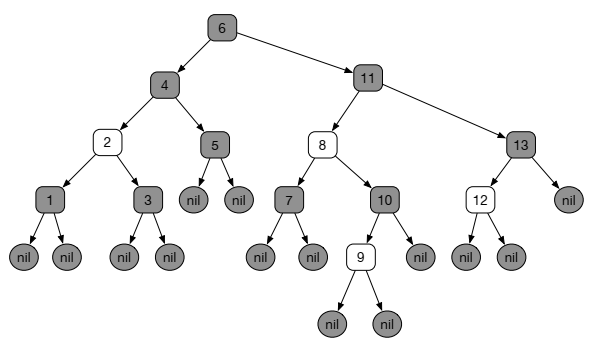
\includegraphics[scale=0.5]{images/lec07-pic15.png}
		\caption{ Красно-чёрное дерево, пример. Красные узлы на рисунке изображены отсутствием заливки}
	\end{figure}
	\[H_{rb} \leq 2\cdot log_2(N)+1\]	
\end{frame}

\begin{frame}[fragile]{Сбалансированное дерево №4. Красно-чёрное дерево}
	\begin{figure}[h]
		\centering
		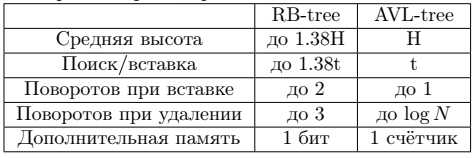
\includegraphics[scale=0.75]{images/lec07-pic16.png}
	\end{figure}
\end{frame}

\section{Дерево отрезков}
  
\begin{frame}
	Пусть нам надо решить задачи:
	\begin{itemize}
		\item многократное нахождение максимального значения на отрезках массива;
		\item многократное нахождение суммы на отрезке массива.
	\end{itemize}	
	Мы умеем совершать эти действия за время $O(N)$, где $N = R - L + 1$. При определённой подготовке можно сократить время на каждую из операций до $O(log N)$.

	~
	
	Для примера возьмём массив:
	\begin{figure}[h]
		\centering
		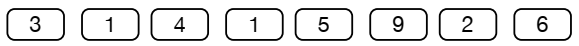
\includegraphics[scale=0.5]{images/lec07-pic17.png}
		\caption{Массив -- основа дерева отрезков}
	\end{figure}
\end{frame}	

\begin{frame}
	Попарно соединим соседние вершины, поместив в узел-родитель значение функции max(left,right). Родитель каждого узла называется \textit{доминирующим узлом}.
	\begin{figure}[h]
		\centering
		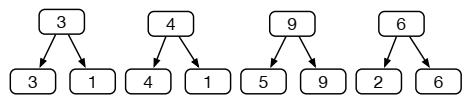
\includegraphics[scale=0.5]{images/lec07-pic18.png}
		\caption{Дерево отрезков: построение. Добавление доминирующих узлов первого уровня}
	\end{figure}
	Проделаем эту же операцию с получившимися узлами:
	\begin{figure}[h]
		\centering
		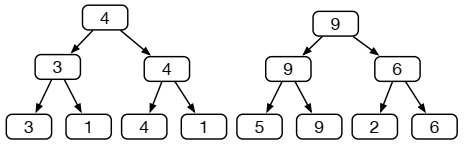
\includegraphics[scale=0.5]{images/lec07-pic19.png}
		\caption{Дерево отрезков: построение. Добавление доминирующих узлов второго уровня}
	\end{figure}	
\end{frame}	

\begin{frame}
	Итог:
	\begin{figure}[h]
		\centering
		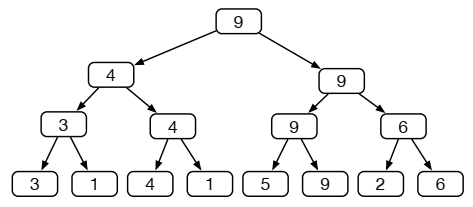
\includegraphics[scale=0.5]{images/lec07-pic20.png}
	\end{figure}
	После построения такого дерева задачу нахождения максимума на отрезке можно решить за $O(log N)$.
\end{frame}	

\begin{frame}
	Дерево отрезков: поиск максимума на отрезке
	\begin{figure}[h]
		\centering
		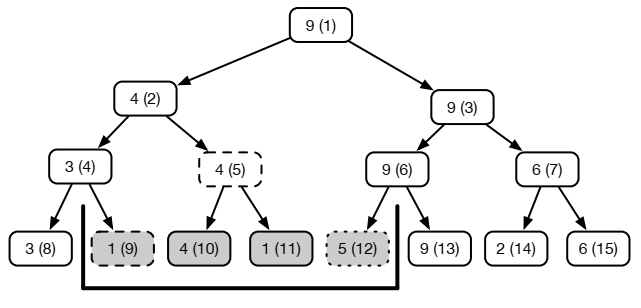
\includegraphics[scale=0.5]{images/lec07-pic21.png}
	\end{figure}
	\begin{itemize}
		\item Идея вычисления проста -- если на отрезке присутствует пара элементов, имеющая общий доминирующий узел, то результатом вычисления функции для этой пары будет предвычисленное значение доминирующего узла. 
		\item Элементы, не входящие в такие пары, могут находиться либо строго на левом конце отрезка, либо строго на правом. Их придётся явно учесть отдельно -- и это мы сделаем, когда будем реализовывать соответствующие операции.	
	\end{itemize}
\end{frame}

\begin{frame}
	\begin{figure}[h]
		\centering
		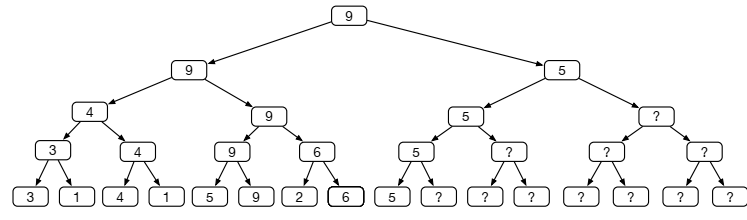
\includegraphics[scale=0.5]{images/lec07-pic22.png}
		\caption{Дерево отрезков: дополнение числа элементов до степени двойки}
	\end{figure}
	Что должно находиться в узлах, отмеченными знаками вопроса?	
	\begin{itemize}
		\item Так как все значения в доминирующих узлах вычисляются с помощью функции P = max(L; R), то то же самое должно происходить с элементом ’?’. 
		\item Это означает, что операция max(L; ?) должна возвращать L. То есть элемент ’?’ есть $\infty$.
		\item Для функции max $\infty$ есть нейтральный элемент.	
	\end{itemize}
\end{frame}

\begin{frame}
	При создании дерева отрезков (Create(size)) создаётся бинарная куча, инициализированная нейтральными элементами. 
	$C$ есть номер первого элемента в нижнем ряду, представляющем заданный набор, над которым будут далее производиться операции. $C = min(2^k) : C > size$
	\begin{figure}[h]
		\centering
		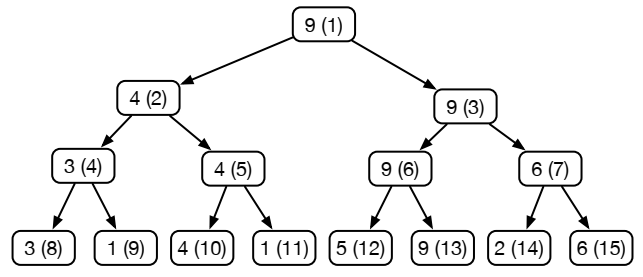
\includegraphics[scale=0.5]{images/lec07-pic24.png}
	\end{figure}	
\end{frame}

\begin{frame}[fragile]
	Каждая операция вставки элемента по сути заменяет нейтральный элемент, который находился в месте вставки, на нужное значение. 
	
	~

	\begin{minted}{c}
Insert/Replace(i, val):
	body[i+C]=val; 
	propagate(i);
	\end{minted}
	
	~
	
	Операция \textit{propagate(i)} рекурсивно обновляет все доминирующие узлы.
\end{frame}

\begin{frame}[fragile]
	Операция нахождения значения функции на интервале [left; right] тоже рекурсивна: 
	
	~

	\begin{minted}{c}
Func(left,right):
	Res = E;
	if (left % 2 == 1) 
		Op(Res, body[left++]);
	if (right % 2 == 0) 
		Op(Res, body[right--]);
	if (right > left) 
		Op(Res, Func(left/2, right/2));
	\end{minted}
\end{frame}

\begin{frame}[fragile]
	Операция создания дерева отрезков требует в худшем случае до $4N$ памяти, а остальные операции имеют логарифмическую сложность.
	\begin{itemize}
		\item Требуемая память: $min=O(2N) .. max=O(4N)$
		\item Операция \textbf{Insert/Replace}: $O(log N)$
		\item Операция \textbf{Func} на любом подотрезке: $O(log N)$	
	\end{itemize}
\end{frame}


\end{document}
